\documentclass[twocolumn]{article}
\usepackage{amsmath,amssymb}
\usepackage{graphicx}


\title{Programming Assignment 1:\\
       Systematically Comparing Motion Planners}
\author{James Marble \\   
        CS 790: Planning Algorithms}
\date{22 February 2010}



\begin{document}
\maketitle

\section{Experiments}

Five planning techniques were tested: PRM, RRT, EST, SBL, and KPIECE. For each of these, three different samplers were tested: uniform, Guassian, and obstacle-based. Because the output of these planners is nondeterministic, 31 runs each were performed with a time limit of 60 seconds each.

\subsection{Environments}

The "Apartment" environment (Fig. \ref{fig:apartment}) provided with omplapp was used in the experiments.  It is complex with many detailed obstacles. The robot is a piano that must be moved to the kitchen. It should be time consuming to check for collisions in this setup.

\begin{figure}
  \centering
    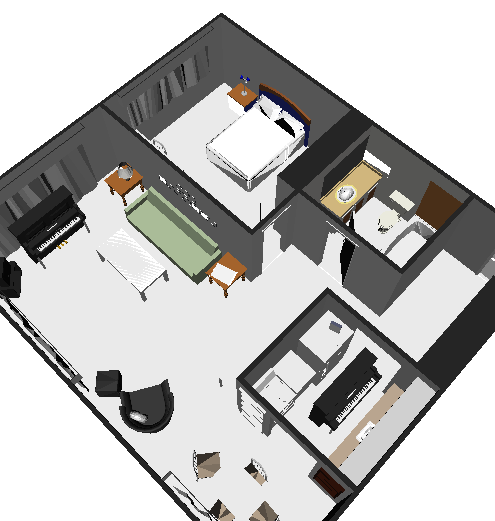
\includegraphics[width=0.4\textwidth]{Apartment}
  \caption{The ``Apartment'' environment and robot.}
  \label{fig:apartment}
\end{figure}

The experiments were also run on the "Easy" environment and robot (Fig. \ref{fig:easy}). None of the variations of experimental parameters showed significant differences in results, however. The remainder of this report details only the results from the "Apartment" environment.

\begin{figure}
  \centering
    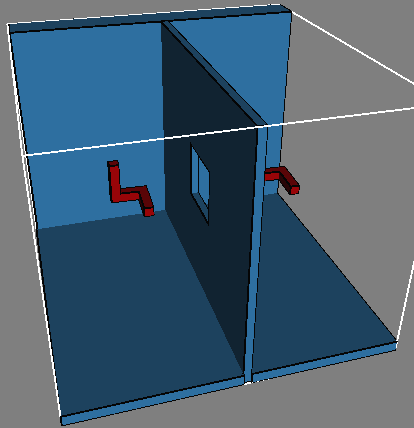
\includegraphics[width=0.3\textwidth]{Easy}
  \caption{The ``Easy'' environment and robot.}
  \label{fig:easy}
\end{figure}

\section{Results}

One technique or sampler does not dominate all others in every measure.

\subsection{Success Rate}

PRM had a low success rate (5-15\%) in this environment. SBL succeeded in finding a solution 50-75\% of the time except with the obstacle-based sampler (5\%).  RRT, EST, and KPIECE all have 100\% success rate.


\subsection{Time}

PRM, RRT, EST all used the maximum available time (60 seconds). For many of the runs (less than half), SBL and KPIECE showed significant speed ups with KPIECE getting as low as 5 seconds while using the obstacle-based sampler.


\subsection{Memory}

Despite having using up to 8-times as many edges as the other methods, PRM used much less memory. Listed in ascending order of memory usage: PRM, RRT, EST, SBL, KPIECE.


\subsection{Solution Length}

When the PRM did find a solution (which was rare), its length was second only to RRT. From there, EST, SBL, and KPIECE had longer solutions (in ascending order).

Smoothing was able to get SBL and KPIECE very close to the length of the PRM solutions and EST was able to be smoothed down to the length of the RRT solutions. The PRM solutions were not improved noticeably by smoothing.

The time to smooth the path was a fraction of a second and the time it took PRM to find that quality of a solution was on the order of a minute. So, path smoothing is very important to get the quality of the faster technique's solution to the level of the slower PRM. The small time investment of smoothing makes it worthwhile in this environment.


\subsection{State Sampler}

The obstacle-based state sampler greatly reduced the number of edges and nodes for all techniques. This translated into slightly reduced memory requirements and time for some of the techniques. The uniform and gaussian samplers showed no significant differences.


\section{Exercises}

\subsection{}

The example benchmark program was modified to accept parameters from a YAML file.
Once the example benchmark was compiling under a separate project, it was trivial (1, 1 hour) to modify it to accept parameters at run time. Actually getting it to link to all the dependencies was slightly more difficult (4, 2 hours).

\subsection {}

The Python script for generating the graphs made analysis of the different planners easy (1, 30 minutes).

\subsection {}

If I could compare the different samplers side-by-side as I could with the planners it would have been easier (2, 30 minutes).

\end{document}
